\chapter[Translating a high-level functional language into the lambda calculus][Translating a high-level functional language into the lambda calculus]{Translating a high-level\\ functional language into the\\ lambda calculus}

In the next few chapters we will describe how to translate a high-level functional language into the lambda calculus. We can regard this translation in two ways:

\begin{numbered}
    \item As a description of the semantics of the language, giving the meaning of each of its constructs in terms of lambda expressions, whose meaning is well understood. This is precisely the approach taken by \textit{denotational semantics} [Gordon 1979].
    \item As a step in the implementation of the high-level language, by expressing all its constructs in terms of the lambda notation.
\end{numbered}

For the sake of definiteness we use a subset of the language Miranda [Turner 1985], but the techniques apply to any functional language. An introduction to Miranda can be found in the Appendix.
\vfill

\plainbox{
    \footnotesize
    {\centering

    \textbf{Disclaimer:}

    }
    \noindent In this book Miranda is used as an example of a modern functional programming language, to illustrate various points about the implementation of functional programming languages in general. This book is not intended to be a source of reference for the definition of Miranda. Note that:
    \begin{numbered}
        \item Miranda has a number of features, both major and minor, which are not discussed here at all.
        \item The material about Miranda in this book was based on a prerelease version of the Miranda system and may therefore be inaccurate by the time it is published.
    \end{numbered}

    The Miranda functional programming system is a product of Research Software Limited, and a full description of the language and its programming environment is in preparation by them.
}

\section{The Overall Structure of the Translation Process}
Miranda is a powerful, high-level functional language, providing a rich set of programming constructs. The purpose of the next few chapters is to demonstrate how some of these constructs can be translated into the lambda calculus. Specifically, we will discuss structured data types, pattern-matching, conditional equations and ZF expressions. Miranda includes a number of other constructs, such as abstract data types and structured data types with laws, which we will not study in this book.

Even so, the translation we describe is a substantial task, and we begin by outlining the structure of the translation process. It might be possible to translate a program directly from Miranda into the lambda calculus, but this would be an extremely complicated translation, so we will take a more step-by-step approach. In order to do this, it is convenient to regard much of the translation as a process of successively \textit{transforming} one program into another, until finally the result is a program in the lambda notation. (We are here using `translation' to suggest a process which takes a program in one language and produces a program in another, while a `transformation' produces a program in the \textit{same} language.)

Two ways of organizing the translation then suggest themselves:

\begin{numbered}
    \item We could perform most of the translation by successive transformations of one Miranda program into another, each transformation performing a simplification step. We would complete the process by translating the resulting (simple) Miranda program into the lambda calculus. The idea is that the earlier transformations would have done all the hard work, so the final step should consist of little more than a change of syntax.

    \item Alternatively, we could begin the translation by performing a simple syntactic translation of the Miranda program into an enriched version of the lambda calculus. This enriched lambda calculus would include the ordinary lambda calculus as a subset, but would also include extra constructs, chosen so that the first step consists of little more than a change of syntax. Then we could do most of the hard work by successively transforming the expression into simpler and simpler forms, until it becomes an ordinary lambda expression, free from any of the extra constructs.
\end{numbered}

Initially, the first method looks more attractive than the second, because it does not require us to define a new language (the enriched lambda calculus). However, we choose to follow the second course of action for the following reasons:

\begin{numbered}
    \item Miranda is designed to be a language for programmers, not compilers, and it lacks certain features that are desirable for a transformation-based compiler. (The particular features lacking are lambda abstractions and the ability to qualify any expression with local definitions. This is not a criticism of Miranda -- it just has a different purpose.)

    \item To a much greater extent than is the case for imperative languages, functional languages are largely syntactic variations of one another, with relatively few semantic differences. Using the second method allows the transformations we present to be applied easily to other languages, by altering only the translation of the high-level language into the enriched lambda calculus.
\end{numbered}

Figure 3.1 depicts the overall plan of action. We will use the term \textit{ordinary lambda calculus} to refer to the language described in Chapter 2, and \textit{enriched lambda calculus} to refer to the language introduced here.

The enriched lambda calculus is simply the ordinary lambda calculus augmented with extra constructs, chosen to allow an easy translation from Miranda. For each construct we will:

\begin{numbered}
    \item say what it looks like (give its syntax);
    \item say what it means (give its semantics).
\end{numbered}

\boxedfigure{
    \centering\sffamily\footnotesize

    \begin{minipage}{10cm}
        \centering

        \framebox{\ Miranda program\ }\\
        \hspace{4cm}$\Bigg\downarrow$ \begin{minipage}{4cm}
            {A simple translation\\ (specific to Miranda)}
        \end{minipage}\\
        \framebox{\
            \begin{minipage}{4.5cm}
                {Expression in the\\ enriched lambda calculus}
            \end{minipage}
            \ }\\
        \hspace{4cm}$\Bigg\downarrow$ \begin{minipage}{4cm}
            {Multiple transformations\\ (independent of Miranda)}
        \end{minipage}\\
        \framebox{\
            \begin{minipage}{4.5cm}
                {Expression in the\\ ordinary lambda calculus}
            \end{minipage}
            \ }\\

    \end{minipage}

}{Translation of Miranda into the lambda calculus}


The semantics for each construct can be given by providing a simple transformation which shows how to express that construct in terms of the ordinary lambda calculus. Then we could, in principle, translate from Miranda into the ordinary lambda calculus by first translating into the enriched lambda calculus, and then using the semantics of each construct repeatedly to transform the expression into an ordinary lambda expression.


While this method generates correct results, far greater efficiency is attainable by using more complicated transformations, but we can always confirm their correctness by reference to the inefficient version.

\section{The Enriched Lambda Calculus}
The enriched lambda calculus is a superset of the ordinary lambda calculus, so that any expression in the ordinary lambda calculus is also an expression in the enriched lambda calculus. The syntax for function application, lambda
abstractions, constants and built-in functions therefore remains exactly as described in Chapter 2. Likewise, all functions are written in prefix form, and the same conventions hold concerning brackets.

The only difference from the ordinary lambda calculus is the provision of four extra constructs. They are:

\begin{numbered}
    \item \ml{let}-expressions and \ml{letrec}-expressions;
    \item pattern-matching lambda abstractions;
    \item the infix operator \fatbar;
    \item case-expressions.
\end{numbered}

Of these, we will only describe the first here. The other three all concern pattern-matching, and cannot be defined before the discussion of pattern-matching itself. This is given in Chapter 4, and the remaining three constructs are defined there.

Figure 3.2 summarizes the syntax of the enriched lambda calculus for future reference.

\subsection{Simple let-expressions}
One of the main constructs in any functional language is the \textit{definition}, whereby a name is bound to a value. This mechanism is provided in the enriched lambda calculus, using \ml{let}-expressions and \ml{letrec}-expressions.

We begin by defining \textit{simple} \ml{let}-expressions. They are called `simple' by contrast with \textit{pattern-matching} \ml{let}-expressions, which we deal with later. A simple \ml{let}-expression has the following syntax:
\begin{mlcoded}
    let v = B in E
\end{mlcoded}

\boxedfigure{
\hspace{-2em}
\begin{tabular}{llll}
    <exp> & ::= & <constant> & Constants \\
          & | & <variable>   & Variables \\
          & | & <exp> <exp>  & Applications \\
          & | & \tl{} <variable> . <exp>   & Lambda abstractions \\
          & | & \ml{let\phantom{rec}} <pattern> = <exp> \ml{in} <exp> & \ml{Let}-expressions \\
          & | & \ml{letrec} <pattern> = <exp>  & \ml{Letrec}-expressions \\
          &   & \phantom{\ml{letrec}} $\cdots$ & \\
          &   & \phantom{\ml{letrec}} <pattern> = <exp>  &  \\
          &   & \ml{in} <exp> & \\
          & | & <exp> \fatbar{} <exp>  & Fat bar \\
          & | & \ml{case} <variable> \ml{of} & \ml{Case}-expression \\
          &   & <pattern>\quad $\Rightarrow$\quad <exp> & \\
          &   & $\cdots$ & \\
          &   & <pattern>\quad $\Rightarrow$\quad <exp> & \\
\end{tabular}

\hspace{-2em}
\begin{tabular}{lllll}
    <pattern> & ::= & <constant> &  & Constant patterns\\
              & |   & <variable> &  & Variable patterns\\
              & |   & <constructor> & <pattern> ,\qquad\qquad  & Constructor patterns\\
              &     &  & $\cdots$  & \\
              &     &  & <pattern>  & \\
\end{tabular}

}{Syntax of enriched lambda expressions}


\noindent where the \ml{v} is a variable, and \ml{B} and \ml{E} are expressions in the (enriched) lambda notation.

It introduces a definition for a variable \ml{v}, which binds \ml{v} to \ml{B} in \ml{E}. The definition is in scope with \ml{E} but not \ml{B}. We say that the `\ml{v = B}' is the \textit{definition of the} \ml{let}, the \ml{v} is the variable \textit{bound by the} \ml{let}, and the \ml{B} is the \textit{definition body}.

For example, consider the following \ml{let}-expression:
\begin{mlcoded}
    let x $=$ 3 in ($*$ x x)
\end{mlcoded}
Intuitively, the value of this expression is found by substituting \ml{3} for \ml{x} in the body \ml{($*$ x x)}, and then evaluating the body, giving the result \ml{9}:
\begin{mlalign}
    & let x $=$ 3 in ($*$ x x)\\
    $\rightarrow$ & $*$ 3 3\\
    $\rightarrow$ & 9
\end{mlalign}

A \ml{let}-expression is an expression like any other, and can be used in the same way as any other expression. For example,
\begin{mlalign}
    & $+$ 1 (let x $=$ 3 in ($*$ x x))\\
    $\rightarrow$ & $+$ 1 ($*$ 3 3)\\
    $\rightarrow$ & $+$ 1 9\\
    $\rightarrow$ & 10
\end{mlalign}

For the same reason, \ml{let}-expresions can be nested:
\begin{mlalign}
    & let x $=$ 3 in (let y $=$ 4 in ($*$ x y))\\
    $\rightarrow$ & let y $=$ 4 in ($*$ 3 y)\\
    $\rightarrow$ & $*$ 3 4\\
    $\rightarrow$ & 12
\end{mlalign}

As a matter of convenience, we also allow ourselves to write multiple definitions in the same let; thus:
\begin{letalign}
    let & x $=$ 3\\
        & y $=$ 4\\
    in  & $*$ x y
\end{letalign}

This expression means precisely the same as the previous one. We define a \ml{let}-expresion with several definitions to mean the same as the nested set of \ml{let}-expresions which defines the same variables in the same order, one per \ml{let}-expresion. (Syntactically, it would have been possible to specify that multiple definitions are separated with semicolons, but layout will suffice for our purposes.)

Earlier in this section we developed an informal reduction rule for \ml{let}-expresions. This involved \textit{substitution} and is very reminiscent of the \tb{}-reduction rule, which also uses substitution. For example, to evaluate
\begin{mlcoded}
    (\tlb{x}$*$ x x) 3
\end{mlcoded}

we substitute \ml{3} for \ml{x} in the body \ml{($*$ x x)}, and then evaluate the body. Generalizing this idea, we can now define the semantics of a simple \ml{let}-expresion as follows:
\begin{mlcoded}
    (let v $=$ B in E) $=$ ((\tlb{v}E) B)
\end{mlcoded}

(We use the symbol $=$ to denote the equivalence of two expressions.) That is all that is needed to define its semantics! By repeated application of this equivalence, we could eliminate all simple \ml{let}-expresions from an expression, in favor of lambda abstractions.

\subsection{Simple \ml{letrec}-expresions}
The syntax of a \textit{simple} \ml{letrec}-expresion is similar to that of a simple \ml{let}-expresion:
\begin{letalign}
    letrec & v$_1 =$ E$_1$ \\
           & v$_2 =$ E$_2$ \\
           & $\cdots$ \\
           & v$_n =$ E$_n$ \\
    in & \\
    & E
\end{letalign}

where the \ml{v$_i$} are variables, and \ml{E}, \ml{E$_1$}, ..., \ml{E$_n$} are expressions in the (enriched) lambda notation. We will sometimes abbreviate `\ml{letrec}-expresion' to `letrec' (and `\ml{let}-expresion' to `\ml{let}'), where no ambiguity arises.

The term `\ml{letrec}' is short for `let recursively', and it introduces possibly recursive bindings for a number of variables \ml{v$_i$}. The difference between \ml{let}s and \ml{letrec}s is that the \ml{v$_i$} are in scope in the \ml{E$_i$} (as well as \ml{E}) of a \ml{letrec}. To take an example, the expression
\noindent
\begin{letalign}
    letrec & factorial $=$ \tlb{n}IF ($=$ n 0) 1 ($*$ n (factorial ($-$ n 1)))\\
    in & factorial 4
\end{letalign}
defines a recursive function \ml{factorial}, and applies it to the argument \ml{4}. The value of the expression is thus \ml{24}.

Like \ml{let}-expresions, \ml{letrec}-expresions can appear embedded anywhere in an expression. Unlike \ml{let}-expresions, however, it is essential to allow multiple definitions in a \ml{letrec}-expresion, so as to permit mutual recursion. This is demonstrated by the following example:
\begin{letalign}
    letrec & f $= \ldots$ f $\ldots$ g $\ldots$ \\
           & g $= \ldots$ f $\ldots$ \\
    in $\ldots$ &
\end{letalign}

Here, \ml{f} refers to itself and \ml{g}, and \ml{g} refers to \ml{f}. This cannot be transformed into a nested pair of \ml{letrec}s, because then either \ml{g} would not be in scope in the body of \ml{f}, or vice versa.

It is easy to provide a semantics for a \ml{letrecs} with only a single definition, using the \ml{Y} operator developed in Section 2.4. In particular,
\begin{mlcoded}
    (letrec v $=$ B in E) $=$ (let v $=$ Y (\tlb{v}B) in E)
\end{mlcoded}
The use of \ml{Y} renders the definition non-recursive, so we can then use a \ml{let}-expresion, whose semantics has already been defined.

The case of multiple definitions requires the use of pattern-matching, and so is postponed until Chapter 6.

\subsection{Pattern-matching let$-$ and \ml{letrec}-expresions}
We will also allow \textit{patterns}, as well as variables, to appear on the left-hand side of definitions in \ml{let}s and \ml{letrec}s. We have not yet defined what a pattern is, so we postpone the topic until Chapter 6. However, a variable is just a simple form of pattern, so simple \ml{let(rec)}-expressions are just simple forms of pattern-matching \ml{let(rec)}-expressions.

\subsection{Let(rec)s versus Lambda Abstractions}
So far we have regarded the ordinary lambda calculus as the target language, into which we will transform the program, and \ml{let(rec)}-expressions as intermediate embellishments. However, there are strong efficiency reasons for including \textit{simple} \ml{let(rec)}-expressions in the target language, rather than transforming them into the ordinary lambda calculus.

Specifically, the transformation of a \ml{let}-expresion
\begin{mlcoded}
    let v $=$ B in E
\end{mlcoded}
into the application of a lambda abstraction
\begin{mlcoded}
    (\tlb{v}E) B
\end{mlcoded}
is using a sledgehammer (lambda abstraction) to crack a nut (\ml{let}-expresions). The lambda abstraction \ml{(\tlb{v}.E)} could be applied to many arguments, but it is in fact only ever applied to one, namely \ml{B}. The generality of lambda abstraction is not required, and the special case (that of application to a unique argument) can be exploited by the more sophisticated compilers described later in this book.

This issue manifests itself in a number of ways:
\begin{numbered}
    \item Miranda is a polymorphically typed language, and in Chapter 8 we give an algorithm for type-checking programs. Unfortunately, it is not possible to type-check the program once it has been transformed into the ordinary lambda calculus, but the addition of simple \ml{let(rec)}-expressions is sufficient to solve the problem.
    \item In all implementations except the very simplest, \ml{let}-expressions can be evaluated very much more efficiently than the corresponding application of a lambda abstraction. This applies to all the implementations described from Chapter 14 onwards.
    \item A related problem is that the transformation of \ml{letrec}-expressions into the ordinary lambda calculus compels us to use \ml{Y} to express recursion. The resulting expression is not an efficient implementation, and a more
    sophisticated compiler may wish to handle recursion in a different way
    (see Chapter 14). Keeping the recursion explicit using \ml{letrec} allows scope
    for these optimizations.
\end{numbered}

To summarize, all our implementations, except the very simplest, will require the program to be transformed into the ordinary lambda calculus augmented with simple \ml{let(rec)}-expressions. This approach makes a dramatic contribution to the efficiency of the resulting implementations. On the other hand, little seems to be gained by augmenting the language still further.

\section{Translating Miranda into the Enriched Lambda Calculus}
A program consists of a set of definitions, together with an expression to be evaluated. To keep these two components of the program separate we will use a box, like this:

\begin{center}
\setlength{\tabcolsep}{18pt}
\renewcommand{\arraystretch}{1.5}
\begin{tabular}{|c|}
    \hline
    Set of definitions \\
    \hdashline
    Expression to be evaluated \\
    \hline
\end{tabular}
\end{center}

\noindent For example, we could compute twice the square of 5 with the following Miranda program:
\begin{center}
\setlength{\tabcolsep}{18pt}
\renewcommand{\arraystretch}{1.5}
    \begin{tabular}{|c|}
        \hline
        \ml{square n $=$ n*n } \\
        \hdashline
        \ml{2 $*$ (square 5)} \\
        \hline
    \end{tabular}
\end{center}

\noindent(Note: Miranda is an interactive language, and defines a `program' to be a set of definitions, while the `expression to be evaluated' is typed by the user. For the rest of this book, however, we will use `program' to mean `a set of definitions together with an expression to be evaluated'.) Proceeding informally, we can translate this Miranda program into the enriched lambda calculus quite easily, to produce the expression
\begin{letalign}
    let &square $=$ \tlb{n}$*$ n n\\
    in &($*$ 2 (square 5))
\end{letalign}

We now introduce some notation to help describe the translation process. Consider the translation of the Miranda expression \ml{(2 $*$ (square 5))} into the lambda expression \ml{($*$ 2 (square 5))}. We may regard this translation process as a \textit{function} \metafn{TE}, which takes the Miranda expression as its input, and produces the lambda expression as its output. We write the translation like this:
\begin{mlcoded}
    \metafnbb{TE}{2 $*$ (square 5)} $\equiv *$ 2 (square 5)
\end{mlcoded}
The double square brackets \doublebracket{} are used to enclose the Miranda expression,
to emphasize that the argument to \metafn{TE} is a \textit{syntactic} object. This convention was used in Chapter 2, but the difference on this occasion is that the result of the translation is a syntactic object also, and we use \ml{$\equiv$} rather than \ml{$=$} to remind us of this fact. We call \metafn{TE} a \textit{translation scheme}.

We also need another translation scheme \metafn{TD}, which translates Miranda definitions into definitions suitable for a \ml{letrec}. For example,

\begin{mlcoded}
    \metafnbb{TD}{square n $=$ n*n} $\equiv$ square $=$ \tlb{n}$*$ n n
\end{mlcoded}

Here we see another reason for using \ml{$\equiv$} when writing translation schemes: it avoids confusion with \ml{$=$} symbols in the program being translated. We can now generalize the translation scheme as follows. Given the Miranda program

\begin{center}
    \setlength{\tabcolsep}{18pt}
    \renewcommand{\arraystretch}{1.5}
    \begin{tabular}{|c|}
        \hline
        \ml{\strut Definition$_1$} \\
        $\vdots$\\
        \ml{\strut Definition$_n$} \\
        \hdashline
        \ml{\strut Expression} \\
        \hline
    \end{tabular}
\end{center}
we generate the following (enriched) lambda expression:
\begin{mlcoded}
    letrec \\
    \quad\metafnbb{TD}{Definition$_1$} \\
    \quad$\cdots$ \\
    \quad\metafnbb{TD}{Definition$_n$} \\
    in\\
    \quad\metafnbb{TE}{Expression}
\end{mlcoded}
In the previous example we used a \ml{let} instead of a \ml{letrec}, but Miranda definitions are all potentially recursive, so we must use a \ml{letrec} in general (later work will optimize this--Section 6.2.8).

What we have now done is to reduce the translation problem to one of defining the two translation schemes \metafn{TD} and \metafn{TE}. We will define them for simple cases in the succeeding two sections, and then lay out the plan of the next few chapters, which will extend them to cover more complicated cases.

For the moment, we completely avoid the question of declarations of new types and type-checking. The former will be introduced in Chapter 4 and the latter in Chapter 8.

\section{The \metafn{TE} Translation Scheme}

The translation scheme \metafn{TE} is a function, which takes a Miranda expression as its argument, and produces an equivalent lambda expression as its result, thus:

\begin{center}
    \framebox{\strut\ Miranda expression\ } $\xrightarrow{\qquad\text{\normalsize \metafn{TE}}\qquad}$ \framebox{\strut\ Lambda expression\ }
\end{center}

\noindent We will describe \metafn{TE} by case analysis, giving a rule for each possible form of a
Miranda expression.


\subsection{Translating Constants}
To translate a constant or built-in function is straightforward, assuming that the lambda notation into which we are translating supports the same set of constants. The following rule is all that is required:
\begin{mlcoded}
    \metafnbb{TE}{k} $=$ k
\end{mlcoded}
\noindent where \ml{k} is a constant or built-in function name (we include all Miranda's operators, and literal constants in this category). Thus, for example,

\begin{mlcoded}
    \metafnbb{TE}{5} $=$ 5 \\
    \metafnbb{TE}{$+$} $=$ $+$
\end{mlcoded}

This translation assumes that all the constants and built-in functions have the same names in the lambda notation. It is straightforward to describe changes of name, however. For example, the following set of rules for \metafn{TE} translates the operators $+$, $-$, etc. in Miranda into \ml{PLUS}, \ml{MINUS}, etc.:

\begin{mlcoded}
    \metafnbb{TE}{$+$} $=$ \text{PLUS} \\
    \metafnbb{TE}{$-$} $=$ \text{MINUS}\\
    \normalfont{etc.}
\end{mlcoded}

\subsection{Translating Variables}
An equally simple rule suffices to translate variables:

\begin{mlcoded}
    \metafnbb{TE}{v} $=$ v
\end{mlcoded}
where \ml{v} is a variable (including the names of user-defined functions and constructors).

\subsection{Translating Function Applications}
Function application in Miranda is denoted by juxtaposition, thus \ml{(f x)}. The same syntax is used in the lambda notation, so the rule for translation is simple:
\begin{mlcoded}
    \metafnbb{TE}{E$_1$ E$_2$} $=$ \metafnbb{TE}{E$_1$} \metafnbb{TE}{E$_2$}
\end{mlcoded}
where \ml{E$_1$} and \ml{E$_2$} are arbitrary Miranda expressions. In the case of certain common operators (such as $+$, etc.), Miranda provides infix syntax (that is, the operator is written between its operands). The translation rule to deal with these constructs is:

\begin{mlcoded}
    \metafnbb{TE}{E$_1$ \text{ infix } E$_2$} $=$ \metafnbb{TE}{\text{infix}} \metafnbb{TE}{E$_1$} \metafnbb{TE}{E$_2$}
\end{mlcoded}
where `infix' is an infix operator, and \ml{E$_1$} and \ml{E$_2$} are arbitrary Miranda expressions. We must apply \metafn{TE} to `infix' to accomplish any change of name (see above).

Furthermore, Miranda allows user-defined functions to be used as infix operators by prefixing their names with \$. We can treat this case with the rule

\begin{mlcoded}
    \metafnbb{TE}{E$_1$ \$v E$_2$} $=$ \metafnbb{TE}{v} \metafnbb{TE}{E$_1$} \metafnbb{TE}{E$_2$}
\end{mlcoded}

\subsection{Translating Other Forms of Expressions}
We shall consider two other forms of Miranda expression, namely

\begin{numbered}
\item list expressions such as \ml{[2,5,1]};
\item ZF expressions.

\end{numbered}
We will deal with these in Chapters 4 and 7 respectively.

\section{The \metafn{TD} Translation Scheme}
The \metafn{TD} scheme takes a Miranda definition as its argument and produces a \ml{letrec} definition as its result. We will only give a rather simplified \metafn{TD} scheme here, leaving a more powerful one for later chapters.

There are two cases that we can handle immediately, namely variable definitions and simple function definitions.

\subsection{Variable Definitions}

Consider the Miranda definition
\begin{mlcoded}
    v $=$ 5 $*$ 7
\end{mlcoded}
It can be translated very easily to
\begin{mlcoded}
    v $= *$ 5 7
\end{mlcoded}
All that is required is to translate the body of the definition, using the \metafn{TE} scheme. In general:
\begin{mlcoded}
    \metafnbb{TD}{v $=$ E} $\equiv$ v $=$ \metafnbb{TE}{E}
\end{mlcoded}
where \ml{v} is a variable and \ml{E} is an expression.

\subsection{Simple Function Definitions}
We have already seen an example of translating a simple function definition, when we translated the Miranda definition
\begin{mlcoded}
    \text{square } n $=$ n $*$ n
\end{mlcoded}

\boxedfigure{
    \begin{center}
    \metafnbb{TE}{Exp} translates the expression \ml{Exp}
    \end{center}
    \vspace{-0.5\baselineskip}
    \begin{tabular}{ll}
        \metafnbb{TE}{k} &$\equiv$ \ml{k} \quad\quad (assumes no name-changing) \\
        \metafnbb{TE}{v} &$\equiv$ \ml{v} \\
        \metafnbb{TE}{ E$_1$ E$_2$ } &$\equiv$ \metafnbb{TE}{ E$_1$ } \metafnbb{TE}{ E$_2$ } \\
        \metafnbb{TE}{ E$_1$ infix E$_2$ } &$\equiv$ \metafnbb{TE}{ infix } \metafnbb{TE}{ E$_1$ } \metafnbb{TE}{ E$_2$ } \\
        \metafnbb{TE}{ E$_1$ \$v E$_2$ } &$\equiv$ \metafnbb{TE}{ v } \metafnbb{TE}{ E$_1$ } \metafnbb{TE}{ E$_2$ } \\
    \end{tabular}

\vs
    \begin{tabular}{rll}
        \hspace{1cm} where & \ml{k} & is a literal constant or built-in operator \\
        & \ml{v} & is a variable \\
        & \ml{E$_1$} & is an expression \\
        & \ml{infix} & is an infix operator
    \end{tabular}
    \begin{center}

    \vspace{-0.5\baselineskip}
    \hdashsep
    \vspace{0.25\baselineskip}

    \metafnbb{TD}{Def} translates the definition \ml{Def}
    \end{center}
    \vspace{-0.5\baselineskip}
    \begin{tabular}{ll}
        \metafnbb{TD}{v $=$ E} &$\equiv$ \ml{v} $=$ \metafnbb{TE}{E} \\
        \metafnbb{TD}{ f v$_1$ $\ldots$ v$_n$ $=$ E } &$\equiv$ \ml{f $=$ \tlb{v$_1$}$\ldots$\tlb{v$_n$}\metafnbb{TE}{E}}
    \end{tabular}

\vs
    \begin{tabular}{rll}
        \hspace{1cm} where & \ml{v, v$_i$, f} & are variables \\
        & \ml{E} & is an expression
    \end{tabular}
}{Translation schemes \ml{TE} and \ml{TD} (simple versions)}


\noindent into the \ml{letrec} definition
\begin{mlcoded}
    square $=$ \tlb{n}$*$ n n
\end{mlcoded}

The body of the definition is translated, and a lambda abstraction is generated around it. We can generalize this as follows:
\begin{mlcoded}
    \metafnbb{TD}{f v$_1$ ... v$_n$ $=$ E} $\equiv$ f $=$ \tlb{v$_1$}$\ldots$\tlb{v$_n$}\metafnbb{TE}{E}
\end{mlcoded}
where \ml{f}, \ml{v$_1$}, ..., \ml{v$_n$} are variables and \ml{E} is an expression.

\section{An Example}
We have now shown how to translate a simple subset of Miranda into the enriched lambda notation. Our progress is summarized in Figure 3.3.

To illustrate the translation in action, consider the following Miranda program:
\begin{mlcoded}
    \begin{center}
        %    \setlength{\tabcolsep}{18pt}
        \setlength{\extrarowheight}{0pt}
        \renewcommand{\arraystretch}{.6}

        \begin{tabular}{|l|}
            \hline\\
            average a b $=$ (a $+$ b)/2\\
            \\
            \hdashline \\
            average 2 (3 $+$ 5)\\
            \\
            \hline
        \end{tabular}

    \end{center}
\end{mlcoded}
This will be transformed to:
\begin{mlcoded}
    letrec\\
    \phantom{ww}\metafnbb{TD}{average a b $=$ (a $+$ b)/2}\\
    in\\
    \phantom{ww}\metafnbb{TE}{average 2 (3 $+$ 5)}
\end{mlcoded}
Application of the rules for \metafn{TE} gives
\begin{mlcoded}
    \metafnbb{TE}{average 2 (3 $+$ 5)}\\
    $\equiv$ \metafnbb{TE}{average} \metafnbb{TE}{2} \metafnbb{TE}{3 $+$ 5}\\
    $\equiv$ average 2 (\metafnbb{TE}{$+$} \metafnbb{TE}{3} \metafnbb{TE}{5})\\
    $\equiv$ average 2 ($+$ 3 5)
\end{mlcoded}
Similarly, the rules for \metafn{TD} give
\begin{mlcoded}
    \metafnbb{TD}{average a b $=$ (a$+$b)$/$2}\\
    $\equiv$ average $=$ \tlb{a}\tlb{b}\metafnbb{TE}{(a $+$ b)/2}\\
    $\equiv$ average $=$ \tlb{a}\tlb{b}(\metafnbb{TE}{$/$} \metafnbb{TE}{a $+$ b} \metafnbb{TE}{2})\\
    $\equiv$ average $=$ \tlb{a}\tlb{b}($/$ (\metafnbb{TE}{$+$} \metafnbb{TE}{a} \metafnbb{TE}{b}) 2 )\\
    $\equiv$ average $=$ \tlb{a}\tlb{b}($/$ ($+$ a b) 2)
\end{mlcoded}
Putting it all together gives the result of the translation:
\begin{mlcoded}
    letrec\\
    \phantom{ww}average $=$ \tlb{a}\tlb{b}($/$ ($+$ a b) 2)\\
    in\\
    \phantom{ww}average 2 ($+$ 3 5)
\end{mlcoded}

To complete the example, let us transform the expression into the ordinary lambda calculus. Let us suppose that we spot that the \ml{letrec} may be replaced with a let, because the definition is non-recursive (the method is described in Chapter 6). Then we can use the semantics of \ml{let}-expresions to produce the ordinary lambda expression
\begin{mlcoded}
    (\tlb{average}(average 2 ($+$ 3 5))) (\tlb{a}\tlb{b}($/$ ($+$ a b) 2))
\end{mlcoded}
You can see why we prefer to write programs in Miranda!

\section{The Organization of Chapters 4--9}

In the interests of simplicity, the equations for \metafn{TD} and \metafn{TE} given in Figure 3.3 are far from comprehensive. The rest of Part I of the book is devoted to filling in the details.

Chapter 4 introduces structured data objects, pattern-matching and conditional equations, and gives a simple translation into the enriched lambda calculus. This translation is rather inefficient, and Chapter 5 shows how pattern-matching can be compiled far more efficiently. Chapter 6 then shows how to transform all the constructs of the enriched lambda calculus into the ordinary lambda calculus.

Miranda contains constructs called ZF expressions (also known as list comprehensions). We discuss their translation in Chapter 7.

Finally, Miranda is a polymorphically typed language, and we have so far paid no attention to the question of type-checking. This is addressed in Chapters 8 and 9.

The organization of these chapters is depicted in Figure 3.4.

\begin{figure}[H]
    \centering

    \fbox{%
            \begin{minipage}{0.9\textwidth}
                \small
                \setlength{\parindent}{10pt}
                \setlength{\parskip}{0mm plus 0mm minus 0mm}

                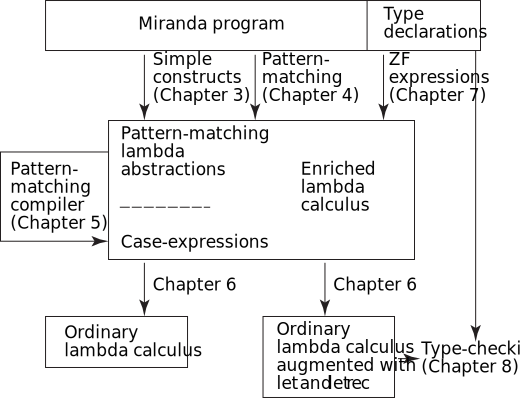
\includegraphics[width=0.96\textwidth]{chapters/Fig3_4}
%                    \includesvg{chapters/Fig3_4}
%                    \input{chapters/Fig3_4.tex}

            \end{minipage}%

    }%

    \caption{\textsf Organization of Chapters 4-8}
\end{figure}

\section*{References}

\begin{references}
    \item Gordon, M.J.C. 1979. \textit{The Denotational Description of Programming Languages}. Springer Verlag.
    \item Turner, D.A. 1985. Miranda -- a non-strict functional language with polymorphic types. In \textit{Conference on Functional Programming Languages and Computer Architecture, Nancy}, pp. 1-16, Jouannaud (editor). LNCS 201. Springer Verlag.
\end{references}
